\chapter{関係データベースの設計と問い合わせの例 -- 研究発表プログラムの管理システム}

これまでの章では，関係データモデルの基本概念，実体関連モデルと正規化理論による関係データベースの設計方法，SQLによる関係データベースへの問い合わせ手法，問い合わせ高速化のための索引づけについて説明してきました．
最終章では，断片的に学んできた関係データベースの知識を総動員して，ある関係データベースの設計と問い合わせの例を見ていきましょう．

\section{問題設定}
最終章でも山畑さんに登場してもらいましょう．
以下は，架空の人物である山畑さんのその後のストーリーです．

\begin{framed}
ショッピングサイトの運営を始めて6年．
運営開始当初の山畑さんは，データベースといえば「大量のデータの集まり」くらいの認識しかなく，Excelシートに蓄積された販売履歴は「データベース」と呼ぶにはあまりにもずさんなものだった．
データには誤りも多く，例えば販売価格がマイナスになっているレコードもあった．
さらに，同じ商品なのに販売単価が異なるなど，データ間で食い違いがあるレコードも散見された．

そんな「データベース（笑）」を使ってデータ分析を行おうとしていた自分を恥ずかしく思えるほど，今の山畑さんは関係データベース設計についての確かな知識と経験を身につけている．
ショッピングサイトに関係データベースを導入して以降，販売履歴をはじめとする様々なデータを正しく管理できるようになった．
また，蓄積された大規模データと分析技術を駆使して，様々なAIサービスも提供できるようになった．
今では，本業のショッピングサイト事業とは別に，データベース設計の受託業務も行うようになり，データベースを活用したウェブサイト作りの巧さではちょっとした話題になっている．

ある日のこと，そんな絶好調の山畑さんのところに，知り合いの大学研究者から「学術フォーラムの申し込みサイト作り」に関する相談が舞い込んだ．
彼曰く，自身が関わっている研究領域が注目を集めており，学術フォーラムの発表者数もうなぎ登りだという．
実際，昨年の学術フォーラムでは発表者数500人を超えたそうだ．
ところが，フォーラムの申し込みサイトは古いシステムを使っていて，データベースもずさんな状態であり，発表申し込みや発表プログラムの管理が非常に大変だという．
知り合いの研究者は，来年度のフォーラムの実行委員長を務めることが決まったそうで，このままではフォーラムの運営で大変な目に遭うことが目に見えているため，山畑さんに「発表プログラムの管理のためのデータベース設計を手伝ってほしい」と相談してきたのだった．

データベースの設計と分析も生業にしつつある山畑さん．
学術フォーラムの運営のためのデータベース設計の依頼を，二つ返事で引き受けたのだった．
\end{framed}

データベース設計の依頼を引き受けた山畑さんは，データベース設計のための要件定義を行うために，実行委員長を含めた学術フォーラムの運営委員会のメンバーにヒアリングを行いました．
以下は，ヒアリングの結果です．

\begin{framed}
%本学術フォーラムでは，発表者および聴講者は事前にサイト上でユーザ登録を行う必要がある．
本学術フォーラムでは，発表者は事前にサイト上でユーザ登録を行う必要がある．
ユーザ登録の際には，氏名，所属，連絡先メールアドレス，職階（例：学生，研究員，教授）を入力する．
ユーザ登録を行うと，ユーザIDが発行される．

%ユーザ登録を済ませた発表希望者は，サイト上で発表申し込みと参加申し込みを行う．
ユーザ登録を済ませた発表希望者は，サイト上で発表申し込みを行う．
発表者は申込時に，自身の氏名，所属，連絡先メールアドレス，職階に加え，発表のタイトル，共同研究者一覧を入力する．
共同研究者についても，発表者と同様に氏名，所属，連絡先メールアドレスを入力する．
発表申し込みが完了すると，発表IDが発行される．
なお，発表件数の増加に伴い，今回のフォーラムでは発表者一人あたりの発表申し込みは1件に制限することにしたい．
%参加申し込みは，発表申し込みとは別に行う．
%参加申し込みが完了すると，参加IDが発行される．

また，発表者および共同研究者の情報について，すでにデータベース内に存在する場合は，申込者の入力負担を減らすために，登録済みの情報を参照できるようにしたい．
ただし，共同研究者は，必ずしも本サイトにログインするユーザであるとは限らない．
そこで，共同研究者がユーザ登録済みの場合はその情報を参照し，未登録の場合は発表申込時に氏名・所属・連絡先を入力して新たに「研究者」としてシステムに登録（ただしログイン権限はなし）できるようにしたい．

%発表はせず，他人の発表を聞くだけの聴講者は，参加申し込みのみを行う．
%参加申込時には，氏名，所属，連絡先メールアドレスを入力するが，ユーザ登録時に入力した情報と同じであれば，ユーザ登録済みの情報を参照できるようにしたい．

発表申し込みの締め切り後，運営委員会は発表内容のタイトルをもとにプログラムを作成する．
プログラムはセッションごとに構成される．
セッションとは，発表内容のテーマに沿って複数の発表をまとめたものを指し，プログラム管理上，各セッションにはセッションIDとセッション名が割り当てられる．
各セッションにはテーマに近い発表が複数割り当てられ，どの発表も必ずどこかの1つのセッションにのみ割り当てられる（1つの発表が複数のセッションにまたがることはない）．
各発表には，セッション内での発表順を示す番号が割り当てられる．
また，各セッションはフォーラム会場内の特定の部屋で実施される．
セッションの参加人数を把握・調整するため，各セッションがどの部屋で行われるか（部屋ID），およびその部屋の名称と収容人数も併せてデータとして管理したい．

各セッションには座長1名を割り当てる．
座長は，運営委員会が作成した座長候補者リストから選ばれる．
座長は担当するセッションの全発表に対して，1点から5点の間でスコアをつける．

座長候補者リストについても，サイト上で管理する．
座長候補者リストには，候補者の氏名，所属，連絡先メールアドレスを登録する．
この情報は発表申し込みユーザとは独立に管理される．

この学術フォーラムでは，優秀な発表には「優秀発表賞」が授与される予定である．
優秀発表者の選定には，発表に対して座長による評価スコアを用いる．
スコアの上位10件の発表に対して，後日優秀発表賞が授与される予定である．
\end{framed}

\section{実体関連図の作成}
ヒアリングの結果をもとに，実体関連図を作成してみましょう．
実体関連図の作成にあたって，まずは\ref{sec:what-is-er-model}節のコラムで触れた「言語分析に基づく実体関連モデルの抽出法」を使って実体型，関連型，それらの属性の候補を洗い出してみましょう．

ヒアリングの文章から，システムで管理すべきデータに関わる名詞を抽出すると，「ユーザ」「氏名」「所属」「メールアドレス」「職階」「ユーザID」「発表者」「共同研究者」「座長」「座長候補者」「発表」「タイトル」「セッション」「セッションID」「セッション名」「発表順」「部屋ID」「名称」「収容人数」「評価スコア」などが挙げられます．

ここで注目すべきは，人物に関わるデータの扱いです．
ヒアリング結果にはシステムに関わる人物として「発表者（登録ユーザ）」「共同研究者」「座長候補者」が登場します．

まず，発表者と共同研究者について考えます．
システムにログインして発表を申し込む「登録ユーザ」と，ユーザ登録はしていないが氏名や所属だけが記録される「未登録の共同研究者」は，どちらも「氏名」「所属」「連絡先メールアドレス」という共通の属性を持ちます．
そのため，\ref{sec:inheritance}節で説明した汎化・継承の概念を用い，共通の属性を持つ上位実体型として\strong{「研究者」を定義し，その下位実体型として特有の属性（ユーザIDや職階）を持つ「登録ユーザ」}を定義するのが効果的です．

一方で，「座長候補者」についてはどうでしょうか．
ヒアリング結果には「この情報は発表申し込みユーザとは独立に管理される」という明確な要件が指定されています．
そのため，座長候補者は先ほどの「研究者」の下位実体型には含めず，\strong{「座長候補者」}という完全に独立した実体型として定義するのが，要件に忠実なモデリングとなります．

これらを踏まえ，独立した存在として識別可能な「実体型」とその「属性」を整理すると以下のようになります．
\begin{itemize}
    \item 研究者（上位実体）：研究者ID（主キー），氏名，所属，メールアドレス
    \begin{itemize}
        \item 登録ユーザ（下位実体）：ユーザID，職階
    \end{itemize}
    \item 座長候補者：候補者ID（主キー），氏名，所属，メールアドレス
    \item 発表：発表ID（主キー），タイトル，評価スコア
    \item セッション：セッションID（主キー），セッション名，部屋ID，部屋の名称，収容人数
\end{itemize}
なお，各セッションの座長は1名であり，担当セッションの全発表に対してスコアをつけるため，「評価スコア」は各発表に対して1つに定まります．
そのため，関連型ではなく「発表」実体型の属性として持たせることが可能です．

次に，これらの実体間のつながりを表す「関連型」を，動詞に注目して整理します．
\begin{itemize}
    \item 申し込み：登録ユーザと発表の関連．今回の要件では発表は1人1件に制限されているため，1対1の関連となります．

    \item 共同研究：研究者（登録・未登録問わず）と発表の関連．1つの発表に複数の研究者が関わり，1人の研究者が複数の発表に関わるため，多対多の関連となります．

    \item 割り当て：セッションと発表の関連．1つのセッションに複数の発表が含まれ，各発表は必ず1つのセッションに属するため1対多の関連となります．また，この関連型は，どの発表が何番目かを示す「発表順」を属性として持ちます．

    \item 座長担当：座長候補者とセッションの関連．1つのセッションにつき座長は1名であり，1人の候補者が複数のセッションを担当し得るため1対多の関連となります．
\end{itemize}

以上を踏まえて作成した実体関連図は図\ref{fig:forum-er-diagram}のようになります．
\begin{figure}[htbp]
    \centering
    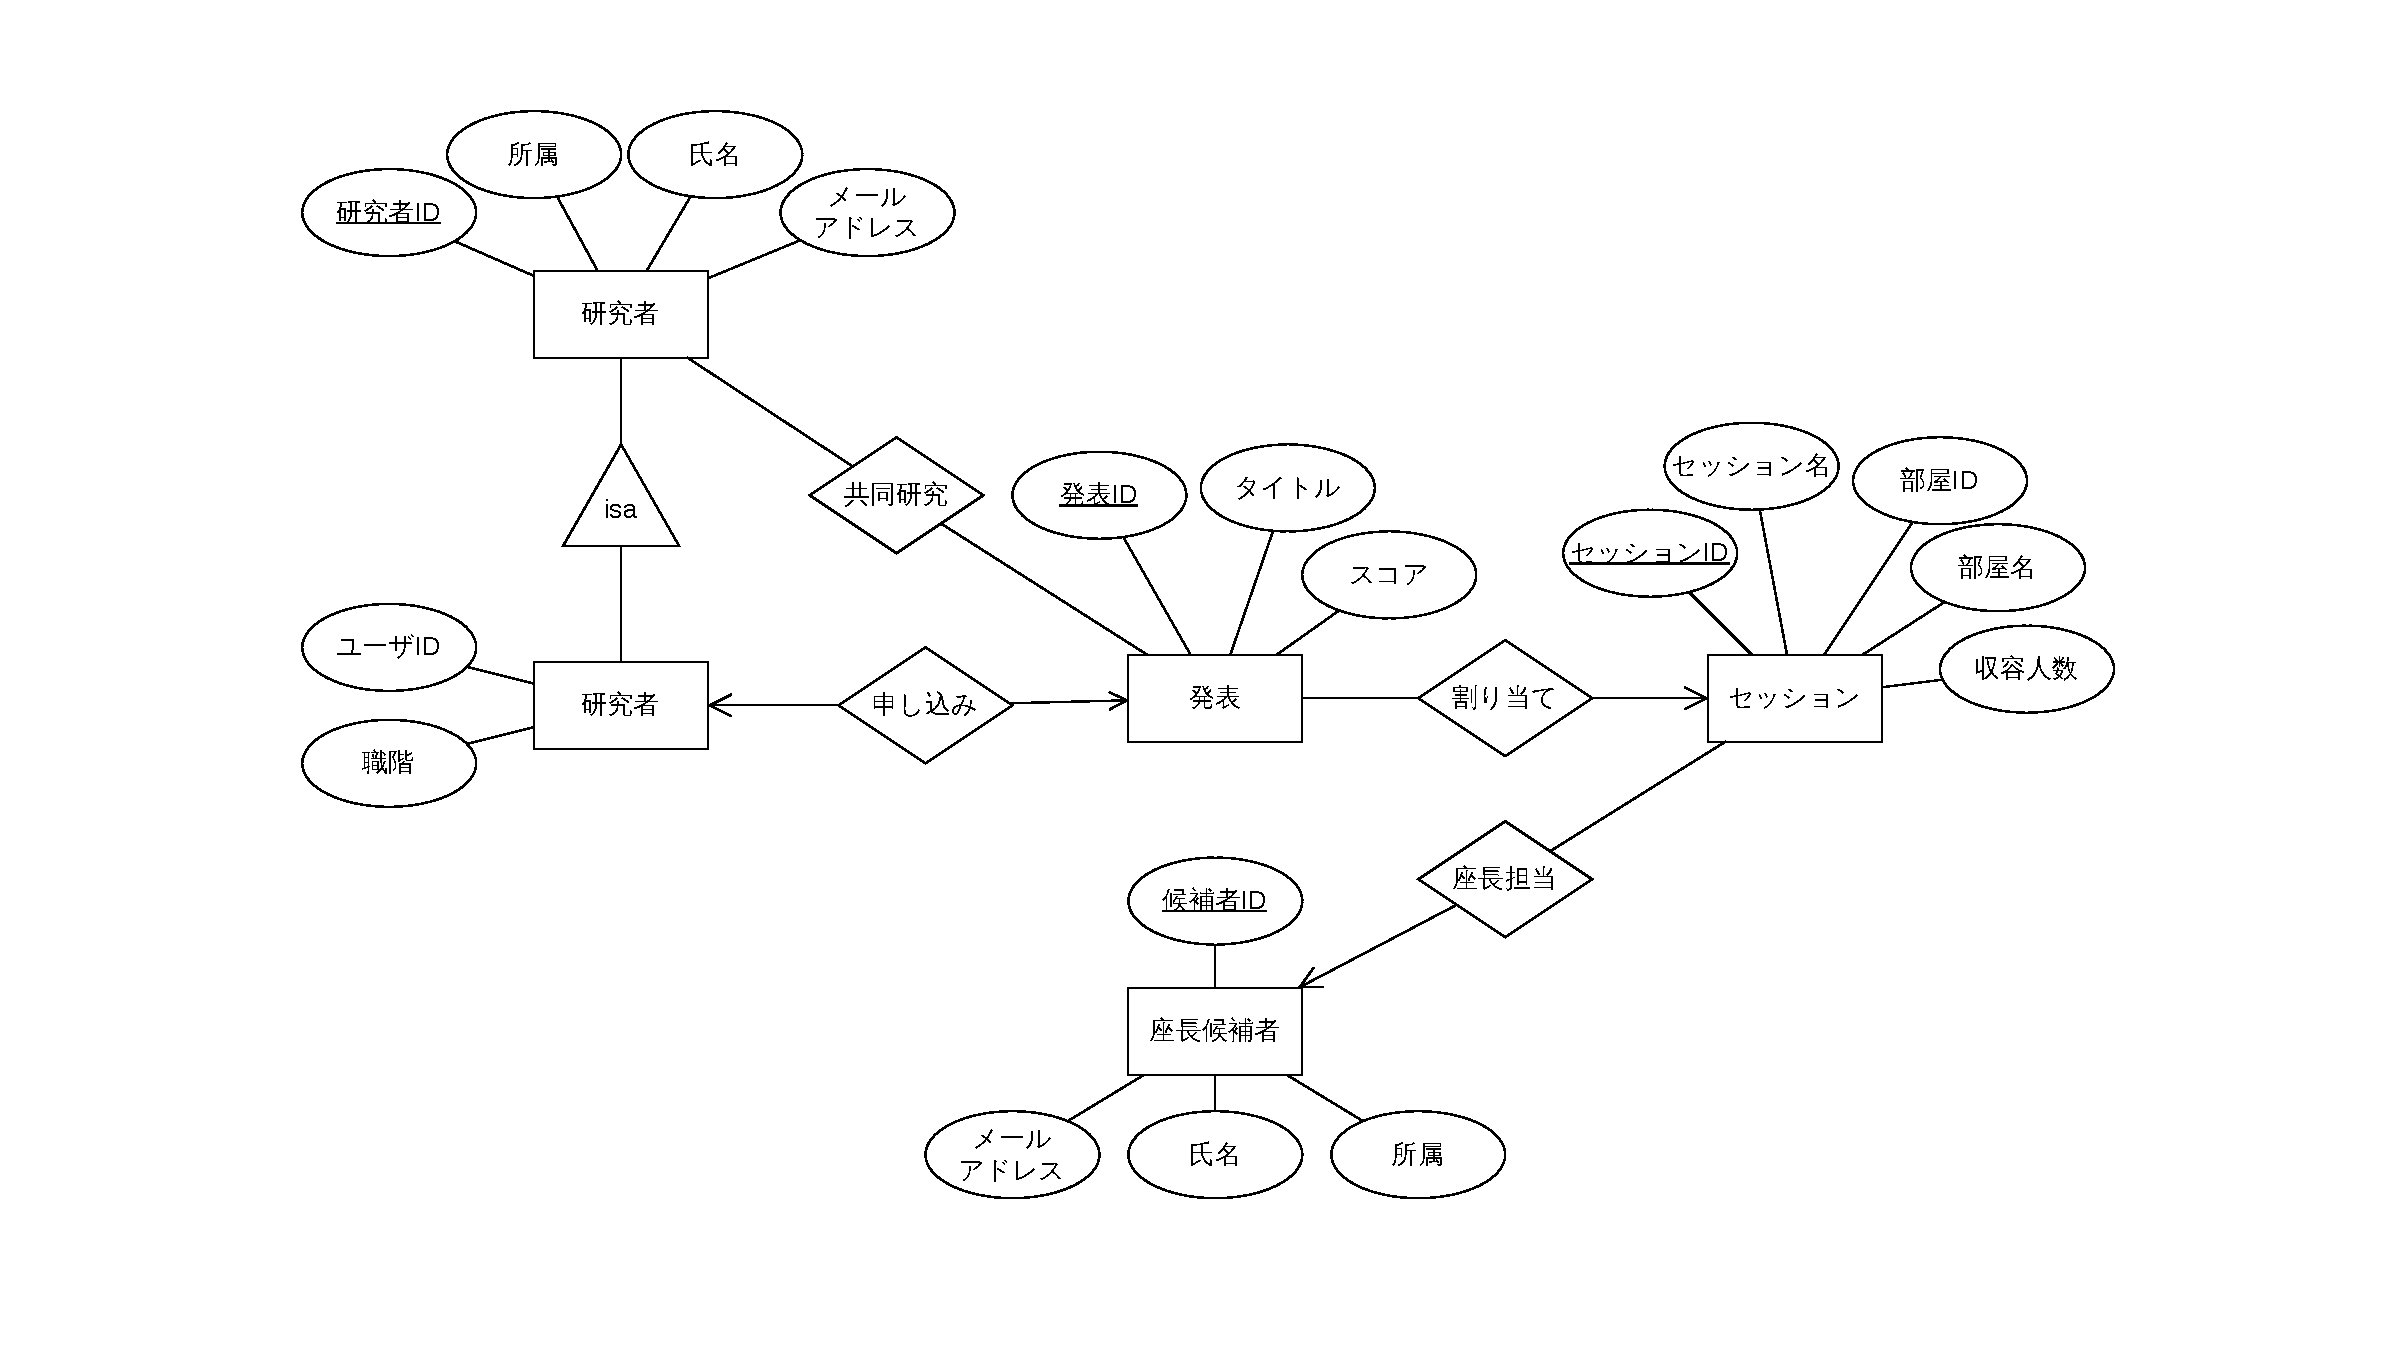
\includegraphics[width=0.99\textwidth]{figure/design-and-analysis-example/forum-er-diagram.drawio.pdf}
    \caption{学術研究フォーラムのデータ管理を行うための実体関連図}
    \label{fig:forum-er-diagram}
\end{figure}


\section{実体関連図から関係スキーマへの変換}
次に\ref{sec:erd-to-relational-model}節で説明した方法を用いて，実体関連モデルを関係データベースで扱うための関係スキーマ（テーブルの定義）へと変換していきます．

まず，汎化・継承を用いた実体型の変換です．
属性の違いを明確に分離し，データの冗長性を防ぐため，別々の関係スキーマに変換するアプローチを採用します．
下位実体型である「登録ユーザ」の関係スキーマは，上位実体型である「研究者」の関係スキーマの主キー（研究者ID）を外部キーとして受け継ぎます．
独立管理される実体型「座長候補者」「セッション」「発表」は，実体関連図上の属性をそのまま関係スキーマの属性とします．

次に，関連型の変換です．
多重度によって変換ルールが異なることに注意して，素直にすべての関連型を関係スキーマに変換してみましょう．
「多対多」の関連である「共同研究」については，両者の主キーを組み合わせた関係スキーマを作成します．
「1対多」および「1対1」の関連については，「多」側（あるいは特定の1側）の主キーを関連型の主キーとし，つながる実体型の主キーを外部キーとして持たせます．
具体的には，以下のようになります．
\begin{itemize}
\item 「1対多」の関連である「割り当て」：「多」側に対応する実体型の主キー（発表ID）を主キーとし，つながる「セッション」の主キー（セッションID）を外部キーとして持たせます．また，関連型が持っていた属性「発表順」も関係スキーマの属性となります．
\item 「1対多」の関連である「座長担当」：「多」側に対応する実体型の主キー（セッションID）を主キーとし，つながる「座長候補者」の主キー（候補者ID）を外部キーとして持たせます．
\item 「1対1」の関連である「申し込み」：今回は実体型「発表」の主キー（発表ID）を「申し込み」の主キーとし，つながるもう一方の実体型「登録ユーザ（研究者）」の主キー（研究者ID）を外部キーとして持たせます．
\end{itemize}

以上，実体関連図を関係スキーマに変換した結果は以下のようになります（簡潔にするため，参照整合性制約を省略しています）．
\begin{align}
&\textbf{研究者}(\underline{\text{研究者ID}}, \text{氏名}, \text{所属}, \text{連絡先メールアドレス}) \\
&\textbf{登録ユーザ}(\underline{\text{研究者ID}}, \text{ユーザID}, \text{職階}) \\
&\textbf{座長候補者}(\underline{\text{候補者ID}}, \text{氏名}, \text{所属}, \text{連絡先メールアドレス}) \\
&\textbf{セッション}(\underline{\text{セッションID}}, \text{セッション名}, \text{部屋ID}, \text{部屋の名称}, \text{収容人数}) \\
&\textbf{発表}(\underline{\text{発表ID}}, \text{タイトル}, \text{評価スコア}) \\
&\textbf{共同研究}(\underline{\text{発表ID}, \text{研究者ID}}) \\
&\textbf{割り当て}(\underline{\text{発表ID}}, \text{セッションID}, \text{発表順}) \\
&\textbf{座長担当}(\underline{\text{セッションID}}, \text{候補者ID}) \\
&\textbf{申し込み}(\underline{\text{発表ID}}, \text{研究者ID})
\end{align}

さて，すべての実体と関連を関係スキーマに変換できましたが，このままではテーブルの数が多く，データを参照するたびに何度も結合（JOIN）を行わなければなりません．
ここで，変換された関係スキーマの「主キー」に注目してみましょう．

関係スキーマ「発表」「割り当て」「申し込み」は，どれも同じ主キー（発表ID）を持っています．
また，「セッション」と「座長担当」も同じ主キー（セッションID）を持っています．
主キーが同じということは，それらのレコードが1対1で対応していることを意味します．
そのため，同じ主キーを持つ関係スキーマの属性を1つの関係スキーマに統合（包含）してしまい，独立した関連のスキーマは削除することができます．

これらを統合した結果，関係スキーマは以下のようにすっきりと整理されます（簡潔にするため，参照整合性制約を省略しています）．
なお，分かりやすくするため，統合した属性名には「座長\_」「発表者\_」などを付与しています．
\begin{align}
&\textbf{研究者}(\underline{\text{研究者ID}}, \text{氏名}, \text{所属}, \text{連絡先メールアドレス}) \\
&\textbf{登録ユーザ}(\underline{\text{研究者ID}}, \text{ユーザID}, \text{職階}) \\
&\textbf{座長候補者}(\underline{\text{候補者ID}}, \text{氏名}, \text{所属}, \text{連絡先メールアドレス}) \\
&\textbf{セッション}(\underline{\text{セッションID}}, \text{セッション名}, \text{部屋ID}, \text{部屋の名称}, \text{収容人数}, \text{座長\_候補者ID}) \\
&\textbf{発表}(\underline{\text{発表ID}}, \text{タイトル}, \text{評価スコア},  \text{発表者\_研究者ID}, \text{セッションID}, \text{発表順}) \\
&\textbf{共同研究}(\underline{\text{発表ID}, \text{研究者ID}})
\end{align}



\section{正規化理論に基づく関係スキーマの修正}
作成した関係スキーマが，データの冗長性を排除し，更新時異状を引き起こさないか，これまでに学んだ正規化理論の観点から確認していきます．

まず，関係スキーマ「発表」と「共同研究者」についてです．
もし「発表」テーブルの中に「共同研究者1」「共同研究者2」といった列を設けてしまうと，ドメインとして原子値以外の値をとることを許す非正規形の関係となり，関係データモデルの出発点である第1正規形に違反します．
前節のスキーマ変換で，多対多の関連から「共同研究者」というテーブルを独立させたのは，まさに第1正規形を満たすための処理だったのです．

次に，関数従属性に注目して，関係スキーマがボイス・コッド正規形もしくは第3正規形を満たしているか点検します．
ここで，関係スキーマ「セッション」に注目してみましょう．
このスキーマには，セッションを実施する部屋に関する情報（部屋ID，部屋の名称，収容人数）が含まれています．
このスキーマ内の属性間に成立する関数従属性を分析すると，主キーである「セッションID」が決まれば，そのセッションが行われる「部屋ID」が一意に決まります．
さらに「部屋ID」が決まれば，その部屋の「部屋の名称」と「収容人数」が一意に決まります．
つまり，以下のような関数従属性が存在します．
\begin{align}
&FD_1: \text{セッションID} \to \text{部屋ID} \\
&FD_2: \text{部屋ID} \to  \text{\{部屋の名称，収容人数\}}
\end{align}

関数従属性$FD_2$の左辺である属性「部屋ID」は，「セッション」テーブルの超キーではありません．
このように，主キーに直接従属しているのではなく，別の属性を経由して間接的に従属している関数従属性が残っている状態は，ボイス・コッド正規形を満たしていません．

もしこのままの設計でシステムを運用し，例えばある部屋の改装工事によって収容人数が変更されたとします．
このとき，その部屋で行われるすべてのセッションのレコードを探し出し，一つ残らず「収容人数」の値を更新しなければなりません．
もし更新漏れがあると，同じ部屋なのにセッションによって収容人数が異なるという更新時異状が発生してしまいます．

このような異状を防ぐため，\ref{sec:FD-lossless-decomposition}節で解説した情報無損失分解の定理に従い，関数従属性の原因（部屋ID）と結果（部屋の名称，収容人数）のセットからなる関係スキーマと，元のスキーマから結果の属性だけを切り離した関係スキーマの2つに分解します．
具体的には，以下のように関係スキーマ「セッション」から「部屋ID」を主キーとする新しい関係スキーマ「部屋」を切り出します．
\begin{align}
&\textbf{セッション}(\underline{\text{セッションID}}, \text{セッション名}, \text{部屋ID}, \text{座長\_候補者ID}) \\
&\textbf{部屋}(\underline{\text{部屋ID}}, \text{部屋の名称}, \text{収容人数})
\end{align}
このように分解することで，部屋の収容人数が変わっても「部屋」テーブルの該当レコードを1箇所更新するだけで済み，更新時異状が発生しないようになります．

なお，要件の最後にあった「スコア平均の上位10件」についてですが，平均値などのデータの集計結果は，独立したテーブルとしては持たせず，SQLの集約関数などを用いて算出するのが定石です．

こうして，すべての要件を満たしつつ，データの重複がなくなり，データを正しく矛盾なく管理・処理できる堅牢な関係データベースの設計が完成しました．
最終的に完成した関係スキーマは以下のようになります．
\begin{align}
&\textbf{研究者}(\underline{\text{研究者ID}}, \text{氏名}, \text{所属}, \text{連絡先メールアドレス}) \\[7pt]
&\textbf{登録ユーザ}(\underline{\text{研究者ID}}, \text{ユーザID}, \text{職階}) \\
&\pi_{研究者ID}(\textbf{登録ユーザ}) \subseteq \pi_{研究者ID}(\textbf{研究者})  \\[7pt]
&\textbf{座長候補者}(\underline{\text{候補者ID}}, \text{氏名}, \text{所属}, \text{連絡先メールアドレス})  \\[7pt]
&\textbf{セッション}(\underline{\text{セッションID}}, \text{セッション名}, \text{部屋ID}, \text{座長\_候補者ID}) \\
&\pi_{部屋ID}(\textbf{セッション}) \subseteq \pi_{部屋ID}(\textbf{部屋}) \\
&\pi_{座長\_候補者ID}(\textbf{セッション}) \subseteq \pi_{候補者ID}(\textbf{座長候補者}) \\[7pt]
&\textbf{部屋}(\underline{\text{部屋ID}}, \text{部屋の名称}, \text{収容人数}) \\[7pt]
&\textbf{発表}(\underline{\text{発表ID}}, \text{タイトル}, \text{評価スコア},  \text{発表者\_研究者ID}, \text{セッションID}, \text{発表順}) \\
&\pi_{発表者\_研究者ID}(\textbf{発表}) \subseteq \pi_{研究者ID}(\textbf{登録ユーザ}) \\
&\pi_{セッションID}(\textbf{発表}) \subseteq \pi_{セッションID}(\textbf{セッション})  \\[7pt]
&\textbf{共同研究}(\underline{\text{発表ID}, \text{研究者ID}}) \\
&\pi_{研究者ID}(\textbf{共同研究}) \subseteq \pi_{研究者ID}(\textbf{研究者}) \\
&\pi_{発表ID}(\textbf{共同研究}) \subseteq \pi_{発表ID}(\textbf{発表})
\end{align}


\section{SQLによる問い合わせの例}
ここでは，設計した関係スキーマに基づき構築した関係データベース（SQLite）のファイルを用いて，実際の問い合わせ例を確認します．
コチラのURL（\url{https://github.com/trycycle/database-textbook/raw/refs/heads/main/dataset/forum.db}）から\graybox{forum.db}という名前のSQLiteファイルをダウンロードし，SQLiteのクライアントツールなどで開いてみてください．
それでは，山畑さんの知り合いの研究者からの要望をもとに，SQLの記述例を見ていきましょう．

\subsection{プログラムの作成に必要な情報の抽出}
この手の学術フォーラムでは，発表者の登録情報やフォーラム事務局が作成したセッション割り当て情報をもとに，フォーラムのプログラムを作成しウェブサイトやパンフレットなどで公開することが一般的です．
プログラムに最低限掲載するべき情報は，以下が挙げられます．
\begin{itemize}
    \item 発表が割り当てられたセッションのセッション名と部屋の名称
    \item セッションの座長の氏名と所属
    \item セッション内における発表の順番
    \item 発表のタイトル
    \item 発表者の氏名と所属
\end{itemize}

構築した関係データベースから以上の情報を抽出するSQLはコード\ref{code:sql-program}のようになります．
テーブルが複数に分割されているため内部結合が多用されていますが，実体関連図の構造をそのままSQLに落とし込むイメージで書いてみると分かりやすいと思います．
なお，プログラム作成上，発表情報はセッションごとにまとめ，各セッション内で発表は発表順に並んでいた方が都合が良いです．
そのため，SQL文の最後で\graybox{ORDER BY}を用いてレコードをソートしています．
\begin{figure}[htb]
    \begin{minted}[gobble=1,
        bgcolor=background,
        fontsize=\small,
        linenos=false]{sql}

    SELECT
        セッション.セッション名,
        部屋.部屋の名称,
        -- 「発表者」の氏名，所属と混同しないよう別名を付けておく
        座長候補者.氏名 AS 座長氏名,
        座長候補者.所属 AS 座長所属,
        発表.発表順,
        発表.タイトル,
        -- 「座長」の氏名，所属と混同しないよう別名を付けておく
        研究者.氏名 AS 発表者氏名,
        研究者.所属 AS 発表者所属
    FROM
        セッション
    -- 「セッション」テーブルと「部屋」テーブルに同じ属性があるのでUSINGを使う
    JOIN
        部屋 USING(部屋ID)
    JOIN
        座長候補者 ON セッション.座長_候補者ID = 座長候補者.候補者ID
    -- 「セッション」テーブルと「発表」テーブルに同じ属性があるのでUSINGを使う
    JOIN
        発表 USING(セッションID)
    JOIN
        研究者 ON 発表.発表者_研究者ID = 研究者.研究者ID
    ORDER BY
        セッション.セッションID, 発表.発表順;

    \end{minted}
    \captionsetup{name=コード}
    \caption{プログラム作成に必要な情報の抽出するSQL文の例}
    \label{code:sql-program}
\end{figure}


\subsection{優秀発表賞の選定に必要な情報の抽出}
山畑さんの知り合いの要望として，座長がつけた評価スコアをもとに優秀発表賞の選定を行いたいというものがありました．
優秀発表賞の選定に必要な情報は，評価スコアの上位10件の発表のタイトルと発表者の氏名，所属，評価スコアとしましょう．

構築した関係データベースから以上の情報を抽出するSQLはコード\ref{code:sql-award}のようになります．
プログラム作成のSQLよりも結合するテーブルが少ないため，SQL文もすっきりしています．
なお，優秀発表賞の選定上，評価スコアの上位10件の発表を抽出する必要があるため，\graybox{ORDER BY 評価スコア DESC}によってレコードを評価スコアの\strong{降順}にソートし，\graybox{LIMIT 10}によって上位10件のレコードだけを抽出しています．
このSQL文の実行結果は表\ref{tab:sql-award-results}のようになります．
\begin{figure}[htb]
    \begin{minted}[gobble=1,
        bgcolor=background,
        fontsize=\small,
        linenos=false]{sql}

    SELECT
        発表.タイトル,
        研究者.氏名 AS 発表者氏名,
        研究者.所属 AS 発表者所属,
        発表.評価スコア AS スコア
    FROM
        発表
    JOIN
        研究者 ON 発表.発表者_研究者ID = 研究者.研究者ID
    ORDER BY
        評価スコア DESC
    LIMIT
        10;

    \end{minted}
    \captionsetup{name=コード}
    \caption{優秀発表賞の選定に必要な情報の抽出するSQL文の例}
    \label{code:sql-award}
\end{figure}
\begin{table}[htb]
    \centering
    \caption{優秀発表賞の選定に必要な情報の抽出するSQL文の実行結果の例}
    \scalebox{0.60}{
    \begin{tabular}{lllr}
    \toprule
    \textbf{タイトル} & \textbf{発表者氏名} & \textbf{発表者所属} & \textbf{スコア} \\
    \midrule
主成分分析を用いた学生の研究モチベーションの潜在因子抽出と意味解析 & 山田 次郎 & 先進学術研究所 & 5.0 \\
自然言語処理を用いた実験機材の稼働ログ・マニュアルからの構造化データ抽出 & 木村 三郎 & データドリブンユニバーシティ & 5.0 \\
Transformerを用いた産学連携パートナー候補のテキストデータからの逸脱異常検知 & 松本 学 & 論文データサイエンス研究所 & 5.0 \\
勾配ブースティングを用いた研究評価マトリクスのスコア予測と評価データの拡張 & 阿部 結衣 & 関東リサーチテック大学 & 5.0 \\
大規模言語モデルを用いた研究費の採択確率予測モデルにおける申請書の異常検知 & 橋本 哲也 & 未来ラボシステムズ & 5.0 \\
$\vdots$ & $\vdots$ & $\vdots$ & $\vdots$ \\
    \bottomrule
    \end{tabular}
    }
    \label{tab:sql-award-results}
\end{table}


もう1つだけSQLの例を見てみましょう．
山畑さんの知り合いは，運営委員会が次年度のプログラム企画の参考にするために「どのセッションが最も盛り上がったか（評価が高かったか）」を分析したいと考えました．
そこで，セッションごとに評価スコアの平均値を算出し，平均スコアが高い順に並べてみましょう．
これを実現するSQL文はコード\ref{code:sql-session-score}のようになります．
評価スコアは「発表」テーブルのレコードに格納されており，\graybox{GROUP BY}を用いてセッションごとにレコードをグループ化し，\graybox{AVG}関数を用いて各セッションの評価スコアの平均値を算出しています．
このSQL文の実行結果は表\ref{tab:session-scores}のようになります．
\begin{figure}[htb]
    \begin{minted}[gobble=1,
        bgcolor=background,
        fontsize=\small,
        linenos=false]{sql}

    SELECT
        セッション.セッション名,
        AVG(発表.評価スコア) AS 平均スコア
    FROM
        セッション
    JOIN
        発表 USING(セッションID)
    GROUP BY
        セッション.セッションID,
        セッション.セッション名
    ORDER BY
        平均スコア DESC;

    \end{minted}
    \captionsetup{name=コード}
    \caption{セッションの評価スコアを算出するSQL文の例}
    \label{code:sql-session-score}
\end{figure}
\begin{table}[htb]
    \centering
    \caption{セッションの評価スコアを算出するSQL文の実行結果の例}
    \scalebox{0.99}{
    \begin{tabular}{lr}
    \toprule
    \textbf{セッション名} & \textbf{平均スコア} \\
    \midrule
オープンサイエンスとデータ共有 (3) & 4.58 \\
論文データの自然言語処理 (4) & 4.52 \\
研究資金・リソースの最適配分 (1) & 4.36 \\
学術コミュニティのネットワーク分析 (10) & 4.24 \\
若手研究者のキャリアモデリング (8) & 4.2 \\
$\vdots$ & $\vdots$ \\
    \bottomrule
    \end{tabular}
    }
    \label{tab:session-scores}
\end{table}
